\documentclass[11pt]{article}
\usepackage[scaled=0.92]{helvet}
\usepackage{geometry}
\geometry{letterpaper,tmargin=1in,bmargin=1in,lmargin=1in,rmargin=1in}
\usepackage[parfill]{parskip} % Activate to begin paragraphs with an empty line rather than an indent %\usepackage{graphicx}
\usepackage{amsmath,amssymb, mathrsfs, dsfont}
\usepackage{tabularx}
\usepackage[font=footnotesize,labelfont=bf]{caption}
\usepackage{graphicx}
\usepackage{xcolor}
%\usepackage[linkbordercolor ={1 1 1} ]{hyperref}
%\usepackage[sf]{titlesec}
\usepackage{natbib}
\usepackage{../../Tianpei_Report}
%\usepackage{appendix}
%\usepackage{algorithm}
%\usepackage{algorithmic}

%\renewcommand{\algorithmicrequire}{\textbf{Input:}}
%\renewcommand{\algorithmicensure}{\textbf{Output:}}



\begin{document}
\title{Lecture 2: Constituency Parsing}
\author{ Tianpei Xie}
\date{ Jun. 27th., 2022 }
\maketitle
\tableofcontents
\newpage
\allowdisplaybreaks
\section{Concepts}
\textbf{Syntactic parsing} is the task of assigning a syntactic structure to a sentence. This chapter focuses on \emph{constituency structures}, those assigned by context-free grammars (CFG). In a sense, it is the process of inferring the \textbf{parse tree} behind the text. Parse trees can be used in applications such as
\begin{itemize}
\item  \textbf{grammar checking}: sentence that cannot be parsed may have grammatical errors (or at least be hard to read). 
\item \textbf{semantic analysis}: as intermediate stage of representation
\item \textbf{question answering}: 
\item \textbf{name entity recognition}:
\end{itemize}

\subsection{Ambiguity in syntatic parsing}
The most serious problem baced by syntactic parser is \textbf{Ambiguity}. 
\begin{itemize}
\item \textbf{part-of-speech ambiguity} and \emph{part-of-speech disambiguation}. \textbf{Words} are ambiguous — \textbf{have more than one
possible part-of-speech}— and the goal of part-of-speech disambiguation is to find the correct tag for the situation. For example, "book" can be a verb ("book that flight") or a noun ("hand me that book"). "That" can be a determiner ("Does that flight serve dinner") or a complementizer (thought that your flight was earlier). The goal of POS-tagging is to resolve these ambiguities, choosing the proper tag for the context.
\item  \textbf{structural ambiguity}. Structural ambiguity occurs when the grammar can assign more than one parse tree to a sentence. Structural ambiguity, appropriately enough, comes in many forms. Two common kinds of ambiguity are \textbf{attachment ambiguity} and \textbf{coordination ambiguity}.
\begin{itemize}
\item \textbf{attachment ambiguity}: if a particular constituent can be attached to the parse tree at more than one place.  Various kinds of adverbial phrases are also subject to this kind of ambiguity. e.g. "We saw the Eiffel Tower flying to Paris". "flying to Paris" can be gerundive-VP whose subject is "the Eiffel Tower"   or it can be an adjunct modifying the VP headed by "saw".
\item \textbf{coordination ambiguity}: Phrases can be conjoined by a conjunction like "and". For example, the phrase "old men and women" can be bracketed as "[old [men and
women]]", referring to "old men" and "old women", or as "[old men]" and "[women]", in which case it is only the men who are old.
\end{itemize}
\end{itemize}  

\begin{figure}
\begin{minipage}[t]{1\linewidth}
  \centering
  \centerline{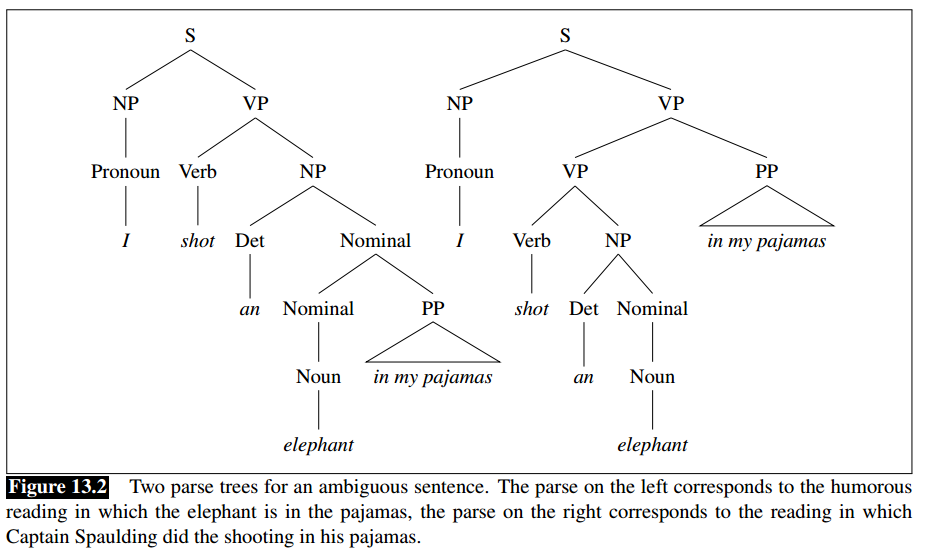
\includegraphics[scale = 0.5]{ambiguitiy_parse.png}}
\end{minipage}
\caption{\footnotesize{\textbf{An example structural ambiguity, i.e. the same sentence can be represented by two parse trees}.}}
\label{fig: structure_ambiguity}
\end{figure}

\section{CKY parsing}
The \textbf{Cocke-Kasami-Younger (CKY) algorithm} is  the most widely used \textbf{dynamic-programming} based approach to syntactic parsing. In dynamic programming, each subproblem represents a parse tree for all the constituents detected in the input.

\subsection{Conversion to Chomsky Normal Form}
The CKY algorithm requires grammars to first be in \emph{Chomsky Normal Form (CNF)}. Note that any context-free grammar can be represented in CNF without lossing information. Let’s start with the process of converting a generic CFG into one represented in CNF. Assuming we are dealing with $\epsilon$-free grammar, there are three situations we need to address in any generic grammar: 
\begin{itemize}
\item rules that \textbf{mix terminals with non-terminals} on the right-hand side: simply introduce a  \textbf{new dummy non-terminal} that covers only the original terminal.
\item rules that have \textbf{a single non-terminal} on the right-hand side, i.e. \textbf{unit productions}. We can eliminate unit productions by rewriting the right-hand side of the original rules with the right-hand side of \emph{all the non-unit production rules} that they ultimately lead to. e.g. if $A \rightarrow B$ by a chain of one or more unit productions and $B \rightarrow \gamma$ is a non-unit production in our grammar, then we add $A \rightarrow \gamma$ for each such rule in the grammar and discard all the intervening unit productions. This leads to flattened rules with a lot of constituents. 
\item rules in which the length of the right-hand side is \textbf{greater than 2}. These are normalized through the introduction of \textbf{new non-terminals} that spread the longer sequences over several new rules.
\end{itemize}

\begin{figure}
\begin{minipage}[t]{1\linewidth}
  \centering
  \centerline{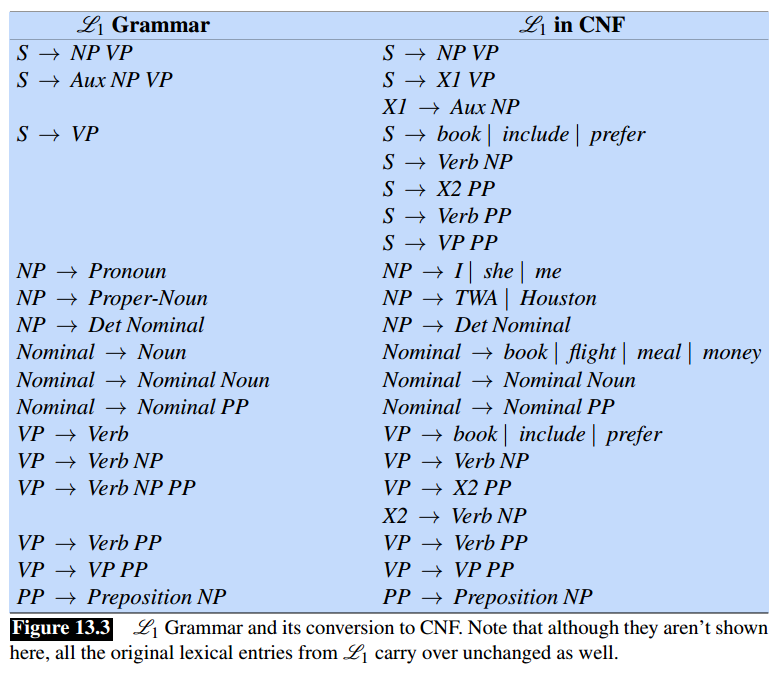
\includegraphics[scale = 0.5]{convert_cnf.png}}
\end{minipage}
\caption{\footnotesize{\textbf{An example grammar conversion to CNF}.}}
\label{fig: cnf_conversion}
\end{figure}

The entire conversion process can be summarized as follows:
\begin{enumerate}
\item Copy all conforming rules to the new grammar unchanged.
\item Convert terminals within rules to \textbf{dummy non-terminals}.
\item Convert \textbf{unit productions}.
\item Make all rules \textbf{binary} and add them to new grammar
\end{enumerate} We can see example in Figure \ref{fig: cnf_conversion}.

\subsection{CKY Recognition}
Following CNF, each non-terminal can have exactly \textbf{two} children except for the last level. Therefore, we can represent the parse tree in a \textbf{two-dimensional matrix}: For a sentence of length $n$, we will work with the \textbf{upper-triangular portion} of an $(n+1) \times (n+1)$ matrix. Each cell $[i, j]$ in this matrix contains the set of \textit{non-terminals} that represent \emph{\textbf{all the constituents that span positions}} $i$ \emph{\textbf{through}} $j$ of the input. i.e. the syntatic parsed structure for substring $s[i:(j+1)]$. The index can be seen as \emph{fenceposts} $"_0\text{ Book }_1 \text{ that }_2\text{ flight }_3$". It follows then that the cell that represents the \emph{entire input} resides in position $[0,n]$ in the matrix.

Note that each non-terminal has two children. So each constituent represented by $[i,j]$ can be decomposed into two parts, i.e. there exists some $k$, $i<k<j$ so that the constituent can be decomposed into those represented by $[i,k]$ and those represented by $[k,j]$. See example in Figure \ref{fig: cky_example}.

\begin{figure}
\begin{minipage}[t]{1\linewidth}
  \centering
  \centerline{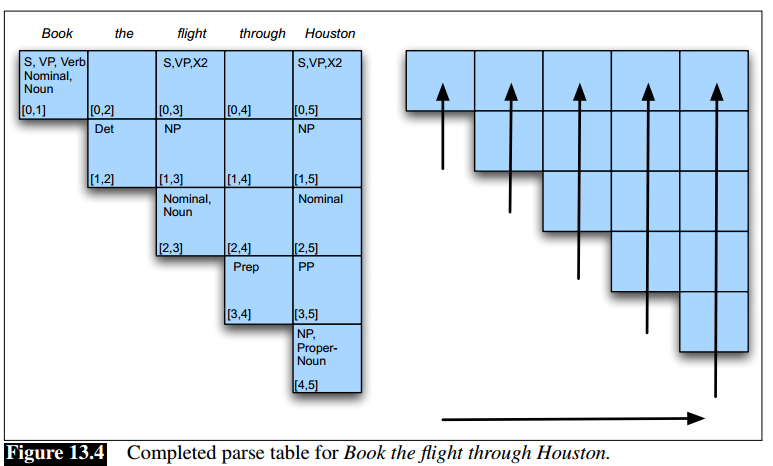
\includegraphics[scale = 0.5]{example_repr_cky.png}}
\end{minipage}
\caption{\footnotesize{\textbf{An example CKY representation}.}}
\label{fig: cky_example}
\end{figure}
\begin{figure}
\begin{minipage}[t]{1\linewidth}
  \centering
  \centerline{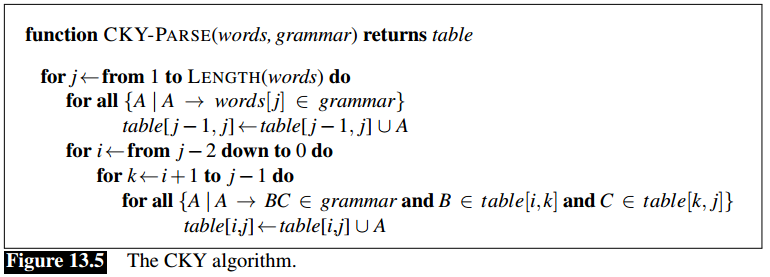
\includegraphics[scale = 0.5]{cky_alg.png}}
\end{minipage}
\caption{\footnotesize{\textbf{The CKY algorithm}.}}
\label{fig: cky}
\end{figure}

Given this reprsentation, the CKY recognition is to fill in the matrix in a bottom-up fashion: before fill in $[i,j]$, we need to fill in all $[i,k], \forall\; k<j$ and $[k,j],\forall\; k>i$, i.e. left to right, bottom to up. The CKY recognition algorithm is described in Figure \ref{fig: cky} \citep{jurafsky2014speech}. Initialization by fill in the diagonal line with all constituents that maps to the single terminal word at $j$. The outer loop is over the columns of matrix and the inner loop is over the rows from diagonal upwards. For each intermediate $[i,j]$, search all $k \in [i+1,j-1]$ and fill in $A$ if there exists rule $A \rightarrow B\;\;C$, where $B \in [i,k]$ and $C \in [k,j]$, i.e. fill in constituent $A$ that can be split by children constituents $B$ and $C$ from its left side and down side, respectively. Finally, if the $[0,n]$ contains the sentence $S$, it means that there exists a valid parse tree in this sentence. 

Note that Algorithm in Figure \ref{fig: cky} is not parser, i.e. it can only \textbf{verify} if a valid parse tree exists in the sentence. One can also find the CKY algorithm in book \citep{skiena2020algorithm} chap. 8.6. 


\subsection{CKY Parsing}
Algorithm in Figure \ref{fig: cky} did not provides the derivation of the sentence, i.e. we do not know how constituents are connected. It turns out that we just need to make some simple modifications so that it can return the parse structure. 
\begin{itemize}
\item the first change is to augment the entries in the table so that each \textbf{non-terminal} is paired with \textbf{pointers} to the table entries from which it was derived, i.e. add links to traverse back from the root to terminals at diagonal position.
\item the second change is to permit multiple \textbf{versions} of the \textbf{same non-terminal} to be entered into the table.
\end{itemize}
Returning an arbitrary single parse consists of choosing an $S$ from cell $[0,n]$ and then\textbf{ recursively retrieving its component constituents from the table}. See example in Figure \ref{fig: cky_parse}. 

In practice, the conversion of CNF may be very complicated to implement. Also our parser isn’t returning trees that are consistent with the grammar given to us by our friendly syntacticians. 

One approach to getting around these problems is to keep enough information around to transform our trees back to the original grammar as a post-processing step
of the parse. This is trivial in the case of the transformation used for rules with length greater than 2. Simply deleting the new dummy non-terminals and promoting their
daughters restores the original tree. In the case of unit productions, it turns out to be more convenient to alter the basic CKY algorithm to handle them directly than it is to store the information needed
to recover the correct trees. 

Note that it takes $\cO(n^2)$ space complexity and $\cO(n^3)$ time complexity to complete parsing, i.e. span though matrix cells takes $\cO(n^2)$ and for each cell, need to scan through all possible split point $k$ which takes $\cO(n)$. 

\begin{figure}
\begin{minipage}[t]{1\linewidth}
  \centering
  \centerline{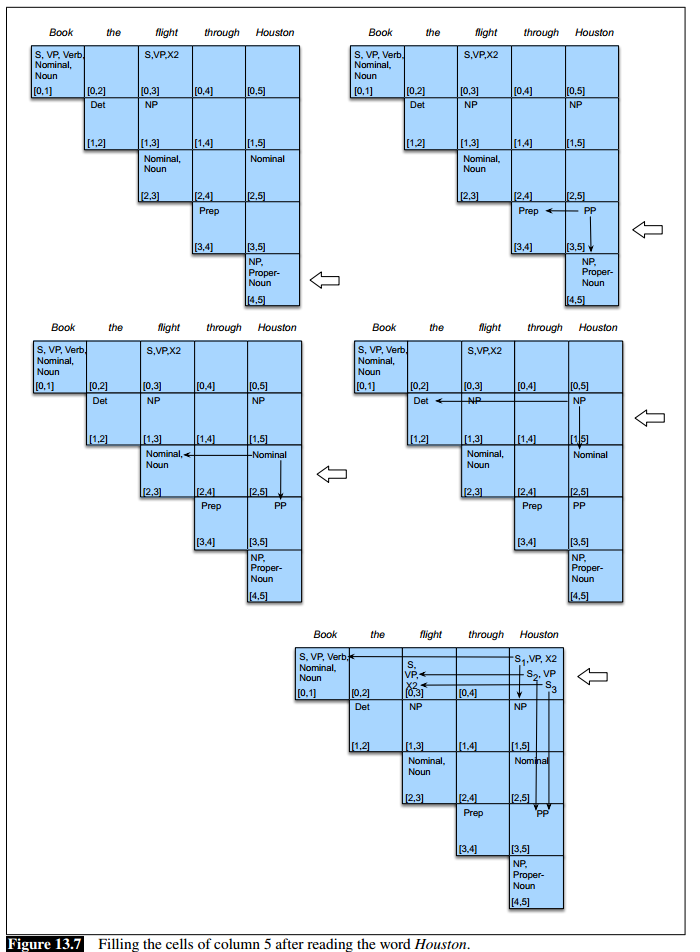
\includegraphics[scale = 0.5]{cky_parsing.png}}
\end{minipage}
\caption{\footnotesize{\textbf{The example of CKY parsing}.}}
\label{fig: cky_parse}
\end{figure}

\section{Neural CKY parsing}
The CKY algorithm doesn't \textbf{disambiguate} among the possible parses, i.e. it does not tell which parse tree is correct. To solve the disambiguation problem we’ll use a simple neural extension of the CKY algorithm \citep{kitaev2018constituency}. The intuition of such parsing algorithms (often called \textbf{span-based constituency parsing}, or \textbf{neural CKY}), is to train a neural classifier to \emph{assign a \textbf{score} to each constituent}, and then use a modified version of CKY to \textbf{combine these constituent scores} to find the \textit{best}-scoring parse tree.



\begin{figure}
\begin{minipage}[t]{1\linewidth}
  \centering
  \centerline{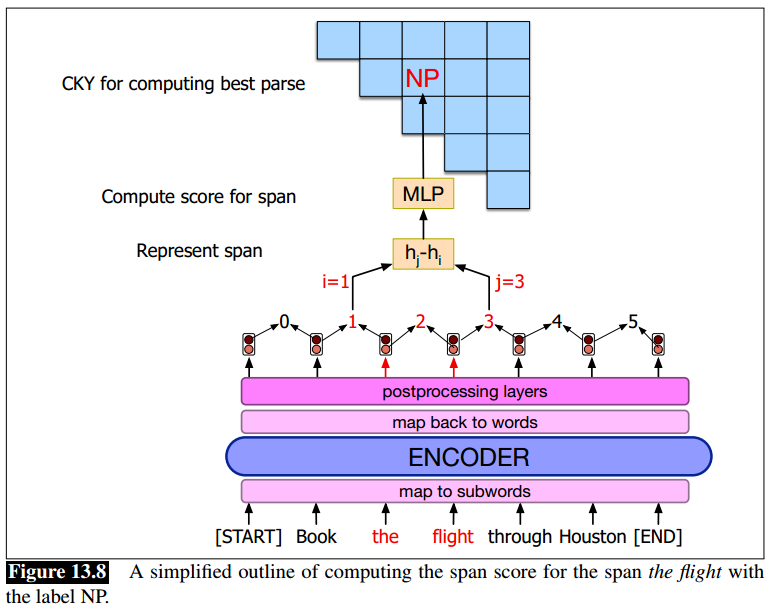
\includegraphics[scale = 0.5]{neural_cky.png}}
\end{minipage}
\caption{\footnotesize{\textbf{The architecture of neural CKY parsing. A score is computed via encoding and mapping of neural network and it is assigned in the matrix of CKY. Then it uses the CKY algorithm to retrieve the optimal path from the root. }.}}
\label{fig: bert_cky_parse}
\end{figure}
\begin{figure}
\begin{minipage}[t]{1\linewidth}
  \centering
  \centerline{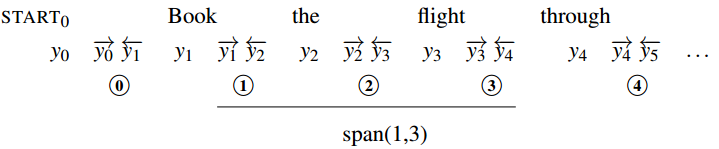
\includegraphics[scale = 0.5]{scan_repr.png}}
\end{minipage}
\caption{\footnotesize{\textbf{The example of scan representation. Each fencepoint has two variables, one scan towards left and one scan towards right}.}}
\label{fig: scan_example}
\end{figure}

\subsection{Computing scores for a Span}
Consider the constituents lie between $words[i:j]$ with non-terminal label $l$, referred as \textbf{\emph{span}}. The goal for the neural network is to \emph{map the span to a score $s(i,j,l)$}. Figure \ref{fig: bert_cky_parse} shows the architecture of neural CKY algorithm. A transformer-based model such as BERT is used to encode the words (sub-words) into embedding representation. (we can map the subword representation back to word representation by looking at the first subword or last subword). The post-processing layers is used after that.

The important step for score computation is to map the word embedding to \emph{\textbf{scan embedding}}. Note that for each position $j$, the scan towards left direction may contain different information from the scan towards right direction. So the \textbf{key} is to encode two values for each position $j$, i.e. define $\overrightarrow{y}_{j}$ as scan beginning with $j$ towards right and $\overleftarrow{y}_{j}$ as scan beginning with $j$ towards left. See Figure \ref{fig: scan_example}. Then the vector \textbf{representation} of scan is computed via difference of embeddings between \emph{start} word and \emph{end} word. It is concatenated for two directions. 
\begin{align*}
v(i,j) &= \brac{\overrightarrow{y}_{j} - \overrightarrow{y}_{i} | \overleftarrow{y}_{j+1} - \overleftarrow{y}_{i+1}}
\end{align*} The scan vector is then passing through a MLP to be converted into a score
\begin{align*}
s(i,j,l) &= \mb{W}_{2,l}\sigma\paren{\text{LayerNorm}\paren{\mb{W}_{1,l}v(i,j)}}
\end{align*} $\sigma(\cdot)$ is the ReLU function. The MLP then outputs a score for each possible non-terminal.

\subsection{Computing scores for a parse tree}
We can represent a parse tree via the scans. Let $T \in \cT$ be a parse tree, 
\begin{align*}
T &= \set{(i_{t},j_{t},l_{t}): \;\; t=1,2,\ldots, |T|}.
\end{align*} This tree is constructed by retrieving the path from root in the CKY matrix. The score for the parse tree can be obtained by computing the sum of all edges in the tree. 
\begin{align*}
s(T)&= \sum_{(i_t, j_t, l_t) \in T}s(i_t, j_t, l_t)
\end{align*} Thus the optimal tree is the one returns maximum scores, $T^{*} = \argmax_{T\in \cT}s(T)$. 

This optimal tree can be found via a variant of CKY algorithm \citep{gaddy2018s}. Here we make some modification of CKY algorithm
\begin{itemize}
\item Define $s_{best}(i,j)$ as the optimal score for sub-tree scanning between $(i,j)$
\item It is easy to compute single-word optimal score i.e. \textbf{diagnoal entries}, i.e. via scanning through all possible non-terminals 
\begin{align*}
s_{best}(i,i+1) &= \max_{l} s(i,i+1,l)
\end{align*}
\item for any $(i,j)$, the following DP-recursion exists:
\begin{align*}
s_{best}(i,i+1) &= \max_{k\in [i+1, j-1]}\brac{s_{best}(i,k) + s_{best}(k,j)} + \max_{l}s(i,j,l).
\end{align*} This has two steps: retrieve best path before it and choose the best current step. 
\end{itemize}


The role of the grammar in classical parsing is to help constrain possible combinations of constituents (NPs like to be followed by VPs). By contrast, the neural model seems to \textbf{learn these kinds of contextual constraints} during its mapping from spans to non-terminals.
\newpage
\bibliographystyle{plainnat}
\bibliography{book_reference.bib}
\end{document}